\documentclass[12pt]{article}
\usepackage[utf8]{inputenc}
\usepackage[T1]{fontenc}
\usepackage[dutch]{babel}
\usepackage{amssymb}
\usepackage{graphicx}
\usepackage{caption}
\usepackage {xcolor}
\usepackage{amsmath}
\usepackage[ruled]{algorithm2e} % linesnumbered: optie om lijnnummers weer te geven
\definecolor {processblue}{cmyk}{0.96,0,0,0}

\usepackage{listings}
\usepackage{color}

\definecolor{dkgreen}{rgb}{0,0.6,0}
\definecolor{gray}{rgb}{0.5,0.5,0.5}
\definecolor{mauve}{rgb}{0.58,0,0.82}

\lstset{frame=tb,
	language=Java,
	aboveskip=3mm,
	belowskip=3mm,
	showstringspaces=false,
	columns=flexible,
	basicstyle={\small\ttfamily},
	numbers=none,
	numberstyle=\tiny\color{gray},
	keywordstyle=\color{blue},
	commentstyle=\color{dkgreen},
	stringstyle=\color{mauve},
	breaklines=true,
	breakatwhitespace=true,
	tabsize=3
}


%opening
\title{Verslag: Practicum TMI}
\author{Andreas Hinderyckx\\ r0760777}
\date{December 2020}

\begin{document}

\maketitle
\newpage

\section{Beschrijving Algoritmen}
\subsection{Brute Force}

\subsubsection{Beschrijving}
De werking van het brute-force algoritme is eenvoudig: elke cirkel uit de invoer wordt op snijpunten gecontroleerd met alle cirkels die nog volgen uit de invoer. Dit leidt tot een tijdscomplexiteit 

\subsubsection{Pseudo-Code}
\begin{algorithm}[H]
	\KwIn{Lijst \texttt{L} met middelpunten en stralen van cirkels}
	\KwResult{Lijst \texttt{S} van alle snijpunten tussen alle cirkels in \texttt{L}}
	\texttt{S} $ \leftarrow \emptyset $\\
	\ForEach{Cirkel \textit{$C_i$} in \texttt{L}}{
		\ForEach{Circkel $ C_j $ in $ \texttt{L}_{>i} $}{
	  		\If{intersection($ C_i $, $ C_j $) != $\emptyset$}{
	  		Voeg snijpunt(en) van $ C_i $ en $ C_j $ toe aan \texttt{S}
  			}
  		}	
	}
\caption{Brute Force-algoritme}
\end{algorithm}
Waarbij de notatie $ \texttt{L}_{>i} $ gebruiken om de cirkels aan te duiden uit de lijst \texttt{L} met een index groter dan \texttt{i}.
\subsubsection{Tijdscomplexiteit}
\textbf{Aanpak analyse tijdscomplexiteit}\\
We bespreken de tijdscomplexiteit in functie van het aantal cirkels uit de invoer, nl.: $ N $. Daar waar in complexiteitsanalyse van sorteeralgoritmes bijvoorbeeld het aantal \texttt{compare}-operaties tussen twee elementen uit de invoer wordt gebruikt als maatstaf voor de uitvoeringstijd, zullen we hier gebruikmaken van het aantal \texttt{intersect}-operaties. Een \texttt{intersect}-operatie krijgt als invoer twee cirkels en berekent het aantal snijpunten tussen deze twee cirkels. De verantwoording achter de \texttt{intersect}-operatie als maatstaf voor de uitvoeringskost te kiezen, is dat deze methode het `duurste' deel is van alledrie de algoritmes. De rest van de algoritmes bestaat uit het opbouwen en doorlopen van gegevensstructuren, wat constant is in kost onafgezien van de grootte van de invoer $ N $. 

\subsubsection{Tijdscomplexiteit Brute Force-algoritme}
Aangezien voor elke cirkel die behandeld wordt, zal vergeleken worden met alle cirkels uit de invoer die op deze huidige cirkel volgen, kunnen we het aantal \texttt{intersect}-operaties als volgt noteren:

\begin{align*}
C &= N + (N-1) + (N-2) + \ldots + 2 + 1\\
&= \dfrac{N(N+1)}{2}\\
&\sim \mathcal{O}(N^2)
\end{align*}


Waarbij we $ C $ gebruiken om de totale kost uit te drukken en gebruikmaakten van de somformule van Gauss: $ \sum_{k=1}^{n} k = \frac{n(n+1)}{2}$ 

\subsection{Naïeve sweepline}
\subsubsection{Beschrijving}

Het idee achter deze naïeve implementatie van een sweepline-algoritme voor het detecteren van snijpunten, is dat we het aantal \texttt{intersection}-oproepen proberen te beperken. Door gebruik te maken van het idee van een (symbolische) sweepline waarbij we de $ x $-as voorstellen als tijds-as, kunnen we ervoor zorgen dat we niet alle cirkels met elkaar moeten vergelijken, maar enkel degene die op een bepaald tijdstip `actief' zijn. Hierbij is een cirkel $ C $ `actief' enkel en alleen indien de sweepline zich op een tijdstip bevindt ná dat de sweepline het meest linkse punt van $ C $ is gepasseerd, en vóór dat de sweepline het meest rechtse punt van $ C $ gepasseerd is. Indien we dit idee implementeren, kunnen we een groot aantal \texttt{intersect}-operaties met cirkels die niet in elkaars buurt liggen vermijden. 

\subsubsection{Pseudo-code}
\begin{algorithm}[H]
	\KwIn{Lijst \texttt{L} met middelpunten en stralen van cirkels}
	\KwResult{Lijst \texttt{S} van alle snijpunten tussen alle cirkels in \texttt{L}}
	\texttt{EventPoints} $\leftarrow$ Gesorteerde lijst \texttt{EventPoints} met start- en eindpunten van alle cirkels\\
	\texttt{S} $ \leftarrow \emptyset $\\
	Lijst \texttt{Actief} $\leftarrow \emptyset$\\
	\ForEach{Punt \texttt{P} in \texttt{EventPoints}}{
		\eIf{\texttt{P} is het begin van een cirkel}{
			\ForEach{Cirkel \texttt{C} in \texttt{Actief}}{
				\If{intersection(\texttt{C}, \texttt{P.Cirkel}) != $\emptyset$}{
					Voeg snijpunt(en) van $ C_i $ en $ C_j $ toe aan \texttt{S}
				}
			}
			Voeg \texttt{C} toe aan \texttt{Actief}
		}{
			Verwijder \texttt{C} uit \texttt{Actief}
		}
	}
	\caption{Naïef sweepline-algoritme}
\end{algorithm}
Waarbij we met \texttt{P.Cirkel} de cirkel bedoelen waarvan het punt \texttt{P} het start- of eindpunt is.
 
\subsubsection{Tijdscomplexiteit}
Een algemene uitdrukking geven voor de tijdscomplexiteit is niet mogelijk voor dit algoritme, aangezien dit sterk afhankelijk is van de ligging van de cirkels. Omwille van deze reden, delen we de analyse op in drie scenario's:
\begin{enumerate}
	\item \textbf{Best case: Disjuncte $ x $-intervallen}\\
		Indien alle cirkels zodanig gepositioneerd zijn dat ze zich allemaal uitstrekken over een interval van $ x $-coördinaten waarbinnen zich geen enkele andere cirkel bevindt, zal het naïeve sweepline algoritme de beste performantie vertonen. In dit geval zal de \texttt{Actief}-lijst namelijk gelijk blijven aan de lege lijst $\emptyset$ doorheen de ganse uitvoering van het algoritme, waardoor er geen enkele \texttt{intersection}-oproep gedaan moet worden. Dit levert een tijdscomplexiteit op die lineair evolueert in het aantal cirkels $ N $: $ \sim \mathcal{O}(N) $  
	\item \textbf{Worst case: gedegenereerd scenario}\\
		Noem de grootste cirkel van de invoer \texttt{C} en stel dat deze een straal \texttt{r} heeft en een middelpunt met $ x $-coördinaat \texttt{x} heeft. Het gedegenereerde scenario waarin alle andere cirkels uit de invoer zich binnen het interval $I = \left[\texttt{x-r}, \texttt{x+r}\right] $ bevinden, is het worst-case scenario voor het naïeve sweepline-algoritme.
		
		 Dit scenario impliceert namelijk dat alle cirkels zich gedurende een bepaalde periode - wanneer de sweepline zich binnen interval $ I $ bevindt - tegelijk in de \texttt{Actief}-lijst zullen bevinden. Hierdoor zal het naïeve sweepline-algoritme reduceren tot het Brute Force-algoritme, aangezien álle cirkels aanwezig zijn in de \texttt{Actief}-lijst en bijgevolg moeten gecontroleerd worden op snijpunten met alle andere cirkels uit de invoer. Dit levert analoog een tijdscomplexiteit op die $ \sim \mathcal{O}(N^2) $ is.
 \item \textbf{Algemeen geval}\\%TODO:concreter bespreken
 		Zoals eerder vermeld, is een algemene uitdrukking geven voor de tijdscomplexiteit van dit algoritme niet mogelijk. Indien we voor de $ x- $ en $ y- $ coördinaten van de middelpunten van de cirkels uitgaan van een uniforme kansverdeling over $ \mathbb{R}^2 $, kunnen we stellen dat het algoritme zich asymptotisch `beter' dan $ \sim \mathcal{O}(N^2) $ zal gedragen, aangezien de kans dat de spreiding van de cirkels zich in een van de twee vorige gevallen bevindt, verwaarloosbaar klein is.
\end{enumerate}

\subsection{Efficiënt sweepline-algoritme}
\subsubsection{Beschrijving}
De werkwijze van het vorige algoritme kan nog verder verfijnd worden. In de vorige implementatie beschouwen we namelijk enkel de $ x $-coordinaten om het aantal \texttt{intersection}-oproepen te beperken en filteren we niet op $ y $-coördinaten. Om dit te kunnen implementeren, moeten we een totale orde op de $ y $-coördinaten van de cirkels definiëren. Aangezien een cirkel echter altijd twee snijpunten heeft met de sweepline \footnote{Behalve op de linker- en rechtereindpunten van de cirkel, waarbij deze twee snijpunten samenvallen}, is het niet voor de hand liggend om deze orde op volledige cirekels te definiëren. 

Om dit probleem op te lossen, splitsen we elke cirkel op in een bovenste en onderste halfcirkel, en nemen we als $ y $-coördinaat voor een halfcirkel de $ y$-coördinaat van het resp. hoogste en laagste punt op de cirkel. Op deze manier kunnen we een totale orde op de halfcirkels definiëren wanneer te sweepline zich op $x$-coördinaat $ a $ bevindt. Deze orde noteren we als: $ <_a $. Door het probleem op deze manier aan te passen, reduceert het probleem zich tot het vinden van snijpunten in een verzameling rechten, waarvoor we het geziene sweepline-algoritme kunnen gebruiken. Dit resulteert dan ook in zeer gelijkaardige code als deze die gezien is in de cursus, zoals is weergegeven in volgende paragraaf. 

\subsubsection{Pseudo-code}
\begin{algorithm}[H]
	\KwIn{Lijst \texttt{L} met middelpunten en stralen van cirkels}
	\KwResult{Lijst \texttt{S} van alle snijpunten tussen alle cirkels in \texttt{L}}
	\texttt{EventPoints} $\leftarrow$ Gesorteerde lijst \texttt{EventPoints} met start- en eindpunten van alle cirkels\\
	\texttt{S} $ \leftarrow \emptyset $\\
	\nl Rood-Zwart-boom \texttt{Actief} $\leftarrow \emptyset$\\\label{alg:sort}
	HalfCirkel boven, onder, huidig\\
	\nl \ForEach{Punt \texttt{P} in \texttt{EventPoints}}{\label{alg:for}
		\eIf{Eventpunt P is een startpunt}
			{
				// \textbf{Geval bovenste halfcirkel}\\
				\texttt{huidig} = bovenste halfcirkel van de cirkel die \texttt{P} omvat\\
				Voeg \texttt{huidig} toe aan \texttt{Actief}\\
				Voeg snijpunten van halfcirkel \texttt{huidig} met \texttt{Boven(Actief, huidig)}
				toe aan \texttt{S}\\
				Voeg snijpunten van halfcirkel \texttt{huidig} met \texttt{Onder(Actief, huidig)}
				toe aan \texttt{S}\\
				
				// \textbf{Geval van onderste halfcirkel}\\
				\texttt{huidig} = onderste halfcrikel van cirkel die \texttt{P} omvat\\
				Voeg \texttt{huidig} toe aan \texttt{Actief}\\
				Voeg snijpunten van halfcirkel \texttt{huidig} met \texttt{Boven(Actief,huidig)}
				to aan \texttt{S}\\
				Voeg snijpunten van halfcirkel \texttt{huidig} met \texttt{Onder(Actief, huidig)}
				toe aan \texttt{S}\\
			}
			{
				// $\text{\textbf{\underline{Eventpunt P is een eindpunt}}}$\\
				// \textbf{Geval bovenste halfcirkel}\\
				\texttt{huidig} = bovenste halfcirkel van de cirkel die \texttt{P} omvat\\
				Voeg snijpunten van \texttt{Boven(Actief, huidig)} en \texttt{Onder(Actief, huidig)}
				aan \texttt{S} toe\\
				Verwijder \texttt{huidig} uit \texttt{Actief}\\
				
				// \textbf{Geval onderste halfcirkel}\\
				\texttt{huidig} = onderste halfcirkel van de cirkel die \texttt{P} omvat\\
				Voeg snijpunten van \texttt{Boven(Actief, huidig)} en \texttt{Onder(Actief, huidig)}
				aan \texttt{S} toe\\
				Verwijder \texttt{huidig} uit \texttt{Actief}\\
			}
	}
	\caption{Sweepline-algoritme}
\end{algorithm}
waarbij de methodes \texttt{Boven(T,c)} en \texttt{Onder(T,c)} de methodes zoals in de cursus zijn die respectievelijk de buur boven \texttt{c} in data-structuur \texttt{T} en de buur onder \texttt{c} in data-structuur \texttt{T} teruggeven.


Om de actieve half-cirkels bij te houden, moeten we gebruik maken van een data-structuur die \textit{insert}- en \textit{delete}-operaties in logaritmische tijd kan uitvoeren, om binnen de perken van de gevraagde tijdscomplexiteit te blijven. Hiervoor maken we gebruik van een Rood-Zwart-boom: een binaire boomstructuur die zichzelf balanceert en waarvan we bijgvolg kunnen afleiden dat ze deze operaties in de gewenste logaritmische tijd kan uitvoeren. In \textit{Java} wordt deze structuur geïmplementeerd door de \texttt{TreeMap}-class, waarvan we in de implementatie ook gebruikmaken.

\subsection{Tijdscomplexiteit}
We analyseren het algoritme stap voor stap om de tijdscomplexiteit ervan te bepalen en veronderstellen een input van $N$ cirkels.
\begin{itemize}
	\item  We starten bij lijn \ref{alg:sort}: hier wordt de lijst van eindpunten van de cirkels gesorteerd, met behulp van mergesort weten we dat we dit in $\mathcal{O}(\log N)$ tijd kunnen realiseren.
	\item Op lijn \ref{alg:for} start de \texttt{for}-lus over alle eindupnten van de cirkels: dit zijn er $2N$. Bijgevolg zal deze lus hoogstens $2N$ keer uitgevoerd worden. In deze \texttt{for}-lus worden drie soorten operaties uitgevoerd:
	\begin{itemize}
		\item Ten eerste \texttt{insert-, remove-, Boven-} en \texttt{Onder}-operaties op de Rood-Zwart-boom \texttt{Actief}. Hiervan weten we dat ze alledrie in $\mathcal{O}(\log N)$ tijd kunnen worden uitgevoerd.
		\item  Ten tweede: \texttt{intersect}-oproepen. De uitvoeringstijd hiervan is onafhankelijk van het aantal cirkels $N$, aangezien ze telkens slechts op twee cirkels wordt uitgevoerd, i.e. $\mathcal{O}(1)$
		\item Ten slotte: operaties die de bovenste of onderste halfcirkel genereren die waartoe \texttt{huidig} behoort. Dit kan in constante tijd gebeuren, aangezien voor elk punt uit \texttt{EventPoints} een verwijzing naar zijn `parent'-cirkel wordt bijgehouden: $\mathcal{O}(1)$.
	\end{itemize}
\end{itemize}
We stellen vast dat er één sorteeroperatie plaatsgrijpt ($\mathcal{O}()\log N)$)en dat alle operaties binnen de \texttt{for}-lus hoogstens $2N$ keer worden uitgevoerd. Tussen twee cirkels zijn hoogstens twee snijpunten en op elk gegeven moment kunnen er zich maximaal $N$ cirkels in \texttt{Actief} bevinden. Concreet levert dit ons:
\begin{itemize}
	\item  \textbf{P is een startpunt}\\
	We hebben $6$ operaties van $\mathcal{O}(1)$ (nl. 4 \texttt{intersect}-oproepen en twee creaties van halfcirkels), $4$ Zwart-Rood-boom operaties (\texttt{Boven} en \texttt{Onder}) voor telkens hoogstens $2$ snijpunten en ten slotte $2$ Zwart-Rood-boom operaties voor de twee huidige halfcirkels. Dit levert ons:
	\begin{align*}
	&6 \mathcal{O}(1) + 2 \mathcal{O}(\log N)  + 2 \left(4 \cdot \mathcal{O}(\log N)\right)\\
	&= 10\mathcal{O}(\log N)
	\end{align*} 
	\item \textbf{P is een eindpunt}\\
\end{itemize}


\section{Experimenten}
\subsection{Maatstaf Complexiteit}
Zoals eerder vermeld, hebben we in dit onderzoek de keuze gemaakt om de complexiteit uit te drukken in functie van het aantal \texttt{intersect}-oproepen, i.p.v. de ruwe rekentijd. In dit onderdeel zullen we hiervoor een argumentatie en motivatie geven.

Een eerste zaak die we moeten aantonen is dat in het algemene geval de rekentijd grotendeels bepaald wordt door het aantal \texttt{intersect}-oproepen dat gedaan wordt bij de uitvoering van een algoritme. Theoretisch gezien stamt dit idee van het feit dat de engige twee aspecten van de drie algoritmes die in uitvoeringstijd zullen toenemen naargelang de invoer toeneemt de volgende zijn:
\begin{itemize}
\item  de zoekoperaties in de Rood-Zwart-Boom (enkel van toepassing voor het finale sweep line-algoritme) enerzijds, en
\item  het aantal berekeningen op snijpunten tussen twee cirkels (\texttt{intersect}-oproepen) anderzijds.

Nu maken we de veronderstelling dat van deze twee factoren, het aantal berekeningen op snijpunten het meeste zal doorwegen in de totale benodigde uitvoeringstijd. Om deze veronderstelling te bevestigen, testen we dit experimenteel.
\end{itemize}

\subsection{Opbouw}
Om een diverse opbouw van experimenten op te bouwen, delen we ze op in volgende deel-experimenten die elks een verschillend aspect van de algoritmes proberen toe te lichten:
\begin{itemize}
	\item \textbf{Aantal Cirkels}\\
		In dit eerste experiment analyseren we eenvoudigweg wat het aantal \texttt{intersect}-oproepen is in functie van het aantal cirkels dat als input gegeven wordt. 
	\item \textbf{Positionering Cirkels}\\
		Hier testen we uit hoe verschillende onderlinge liggingen van cirkels ten opzichte van elkaar invloed hebben op de efficiëntie van de algoritmen, zoals we ook hebben besproken in de vorige respectievelijke secties over tijdscomplexiteit.
\end{itemize}

\subsection{Aantal Cirkels}
In dit eerste experiment testen we de drie algoritmes op eenzelfde input, die toeneemt tot een aantal van zo'n $1000$ input-cirkels waarvan de snijpunten moeten gevonden worden:

\begin{center}
	\makebox[\textwidth]{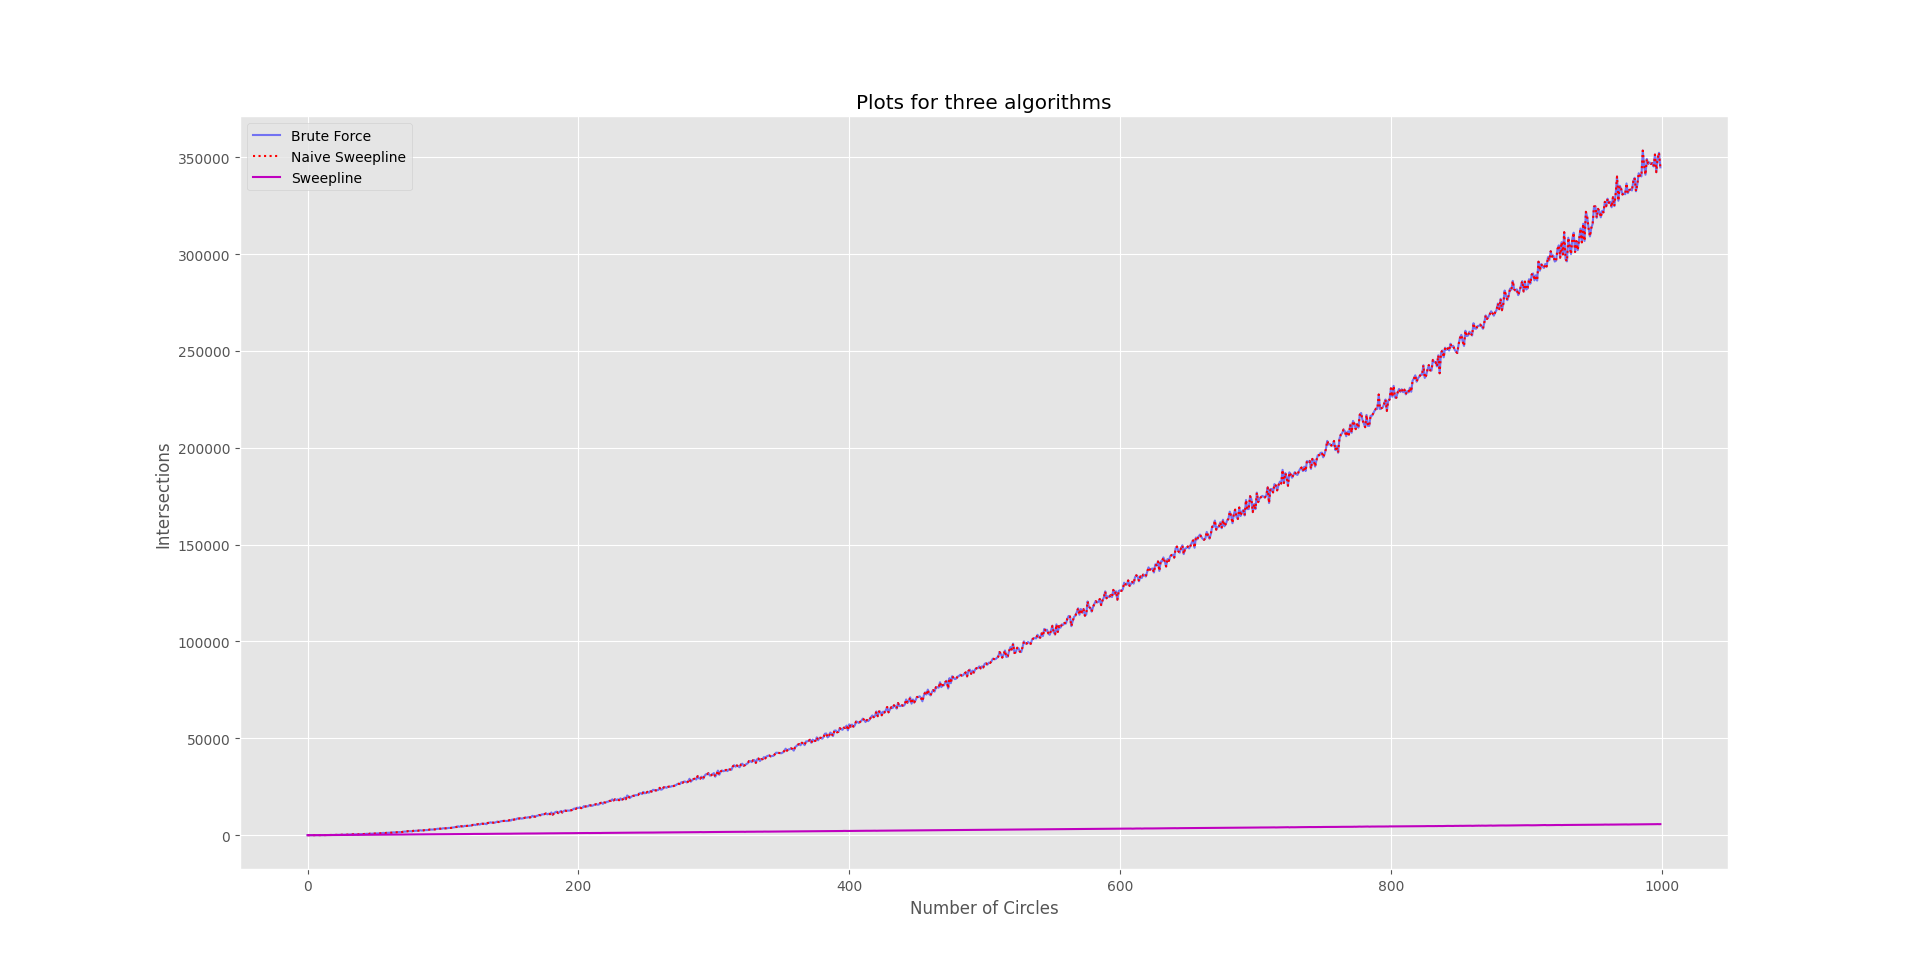
\includegraphics[width=\linewidth]{../plots/ThreeAlgorithmsVisualised}}
\end{center}

Hierbij stellen we vast dat zowel de brute force algoritme als het naïeve sweep line-algoritme een kwadratisch verloop vertonen, qua aantal `intersect'-operaties in functie van het aantal input-cirkels.


%\begin{figure}[h!]
%	\centering
%	
%	\caption[Aantal intersect-operaties in functie van het aantal cirkels]{}
%	\label{fig:variabeleN}
%\end{figure}


\end{document}
